% DOC SETTINGS ===================================
\documentclass{article}
\usepackage[utf8]{inputenc}
\usepackage{steinmetz}
\usepackage{mathtools}  
\usepackage{multicol}
\usepackage{circuitikz}
\usepackage{listings}
\usepackage{geometry}
\usepackage{fancyhdr}
\pagestyle{fancy}
\lhead{ECE2214 Lab Report 2}
\rhead{Kavin Thirukonda 2021}
\fancyheadoffset{0mm}
 \geometry{
 a4paper,
 total={170mm,257mm},
 left=20mm,
 top=25mm,
 }
\mathtoolsset{showonlyrefs} 
\cfoot{}
% DOC SETTINGS ===================================
\begin{document}
\begin{enumerate}
\item Design:
\begin{enumerate}
    \item Hand-written analysis of circuit to design resistors to meet Q-point specifications,and calculate the small-signal voltage gain. 
    \begin{center}
        \ctikzset{bipoles/length=1cm,transistors/scale=1.4,grounds/scale=1.4}
        \begin{circuitikz}[scale=1]
            \ctikzset{tripoles/mos style/arrows}
            \draw (0,0) to [vsourcesin,l=$v_i$](0,2)
            to [R,l=$R_{Si}$](1.5,2)
            to [C,l=$C_{C1}$](3,2)
            to [R,l_=$R_1$] (3,4)
            to [short,-*] (3.75,4)
            to [short, -o](3.75,4.5) node[anchor=south]{$V_{DD}$}
            (3.75,4) to [short,-] (4.5,4)
            to [R,l=$R_D$,-*] (4.5,2.75)
            to [short, -o](5.25,2.75)node[anchor=west]{$v_o$};
            \draw (3,2) to [short,*-] (3.51,2)(4.5,2) node[nmos]{};
            \draw (0,0) to [short, -*] (3,0) to [R,l_=$R_2$] (3,2) 
            (3,0) to [short, -*](4.5,0) node[ground]{} to [short] (4.5,1.22);
        \end{circuitikz}
    \end{center}
    Assume transistor parameters of $V_{TN} = 1.1V, K_n = 100mA/V^2,$ and $\lambda = 0$. Let $V_{DD} = 5V, R_i = R_1||R_2 = 100k\Omega$ and $R_{Si} = 0$. Design the circuit such that $I_{DQ} = 2.5mA$ and the Q-point is in the center of the saturation region.
\end{enumerate}
    \begin{equation}
         I_{Dt} = 2\cdot I_{DQ} = 5mA
    \end{equation}
    \begin{center}
        Now we can use the fact that $V_{DS} = V_{DS}(sat)$ at the transition point to solve for the other value of $V_{DS}$ needed to find $V_{DSQ}$.
    \end{center}
    \begin{equation}
        5mA = 100\frac{mA}{V^2}(V_{DS}(sat))^2 \Rightarrow V_{DSt} = .2236V
    \end{equation}
    \begin{equation}
        V_{DSQ} = \frac{V_{DD}+V_{DSt}}{2}= 2.612V
    \end{equation}
    \begin{center}
        Now we have all the information needed to solve for the resistor values.
    \end{center}
    \begin{align}
        V_{DD} &=  I_{DQ}R_D + V_{DSQ}\\
        \Rightarrow 5V &=  2.5mA\cdot R_D + 2.612V\\
        \Rightarrow R_D &=  \boxed{955.28\Omega}
    \end{align}
    \begin{align}
        2.5mA &= 100\frac{mA}{V^2}(V_{GSQ}-1.1V)^2\\
         V_{GSQ} &= \pm\sqrt{\frac{2.5mA}{100\frac{mA}{V^2}}} + 1.1V\\
         V_{GSQ} &= \underline{1.258V}\text{ or }0.942V
    \end{align}
    \begin{align}
        V_{GSQ} &= V_{DD}\left(\frac{R_2}{R_1+R_2}\right)\\
        \Rightarrow R_1\cdot V_{GSQ} &= V_{DD}(R_1||R_2)\\
        \Rightarrow R_1\cdot1.258V &= 5V\cdot100k\Omega\\
        \Rightarrow R_1 &= \boxed{397.456k\Omega}\\
        \Rightarrow R_2 &= \frac{V_{GSQ}R_1}{V_{DD}-V_{GSQ}}\\
        &= \boxed{133.622k\Omega}
    \end{align}
    \begin{equation}
            A_v = -g_m(r_o||R_D) = -2\sqrt{100\frac{mA}{V^2}\cdot 2.5mA} \cdot 955.28\Omega = \boxed{-30.208}
    \end{equation}
\newpage
\item Simulation:
\begin{enumerate}
    \item Plot $V_i$ and $V_out$ vs time, as simulated by LTspice, displaying the small-signal voltage gain.
    \begin{center}
        \boxed{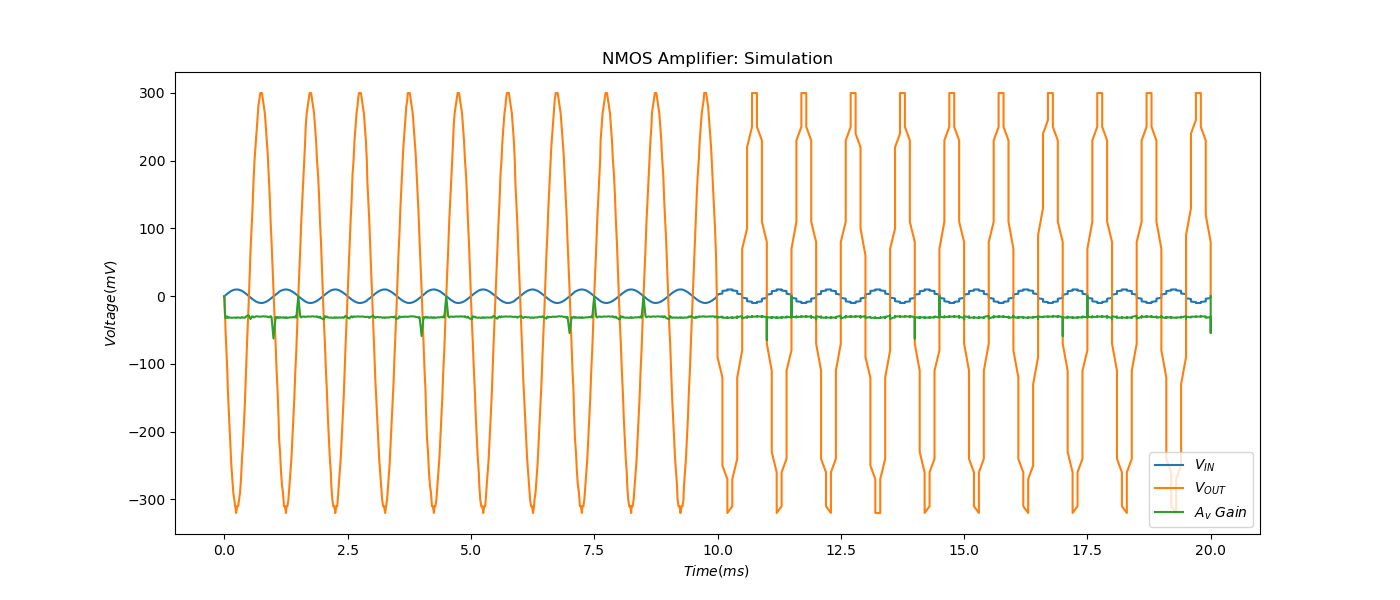
\includegraphics[width = .88\textwidth]{sim.png}}
    \end{center}
    \item List the Q-point $(V_{GSQ}, V_{DSQ}, I_{DQ})$ and small-signal voltage gain (Av) as simulated, and compare to your hand-written analysis.
    \begin{equation}
        V_{GSQ} = 1.26177V
    \end{equation}
    \begin{equation}
        V_{DSQ} = 2.5V
    \end{equation}
    \begin{equation}
        I_{DQ} = 2.617mA
    \end{equation}
    \item Attach a screen shot of your complete LTspice circuit.
    \begin{center}
        \boxed{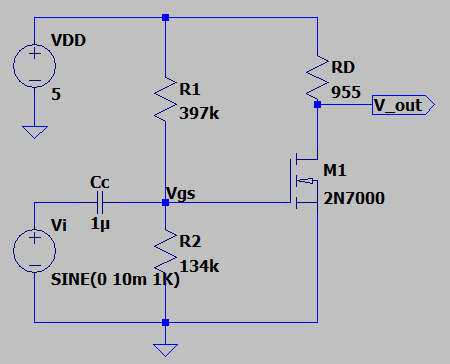
\includegraphics[width = .6\textwidth]{spice.png}}
    \end{center}
\end{enumerate}
\newpage
\item Physical Circuit:
\begin{enumerate}
    \item List the Q-point $(V_{GSQ}, V_{DSQ}, I_{DQ})$ of your physical circuit, as obtained by a multimeter.
    \begin{equation}
        V_{GSQ} = 1.264V
    \end{equation}
    \begin{equation}
        V_{DSQ} = 4.68V
    \end{equation}
    \begin{equation}
        I_{DQ} = 3.5\mu A
    \end{equation}
    \item Plot/screenshot of $V_i$ and $V_{out}$ vs time for the physical circuit,displaying the voltage gain.
    \begin{center}
        \boxed{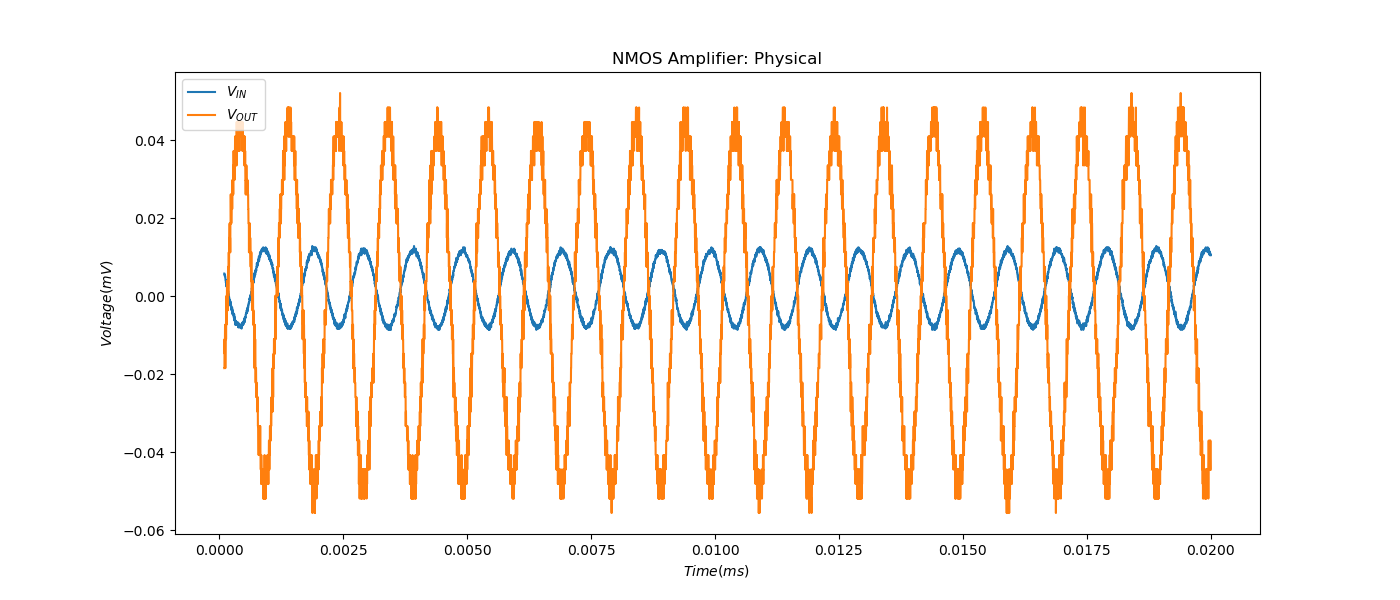
\includegraphics[width = .88\textwidth]{real.png}}
        \boxed{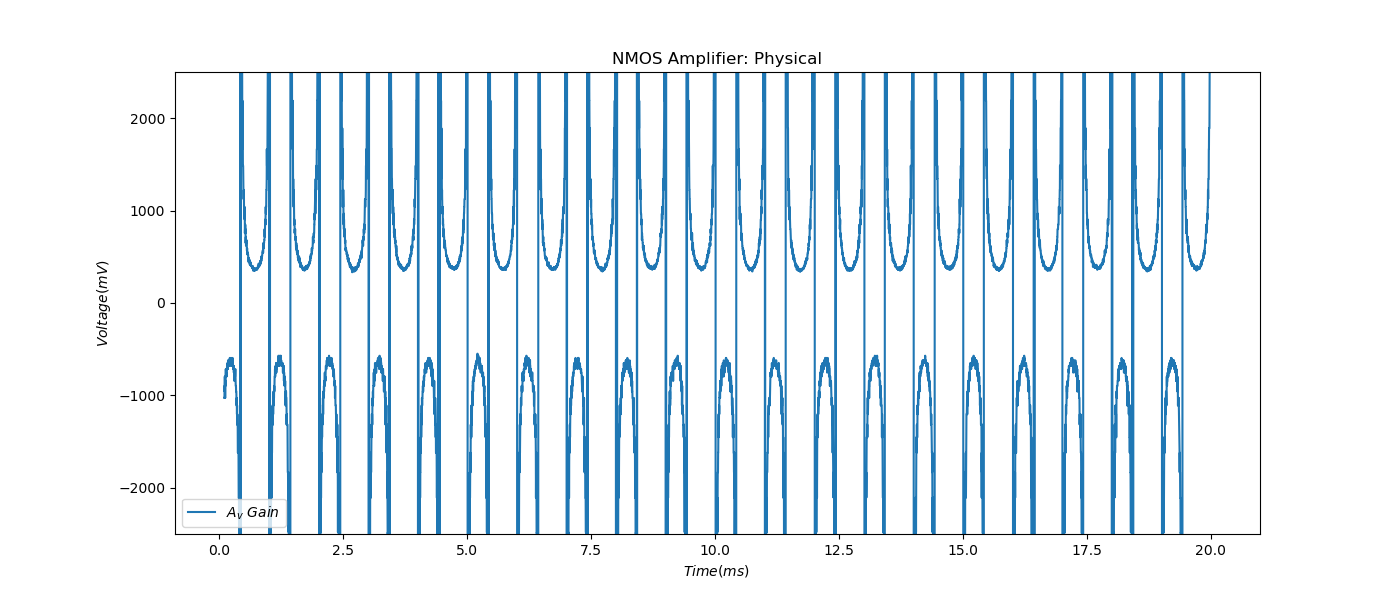
\includegraphics[width = .88\textwidth]{realgain.png}}
    \end{center}
    \begin{center}
        The gain graph is tangential so its output is not very helpful. There is a slight typo in the axis of the first graph, its labeled in milli, when it should be SI unit scale.
    \end{center}
    \item Calculate the small-signal voltage gain by comparing the amplitudes of the two signals.
    \begin{equation}
        A_v = \frac{V_o}{V_i} = \frac{-45}{15} =  -3
    \end{equation}
    \newpage
    \item Using your measurements in parts a)and c), calculate what the actual $K_n$ and $V_{TN}$ parameters are for your physical MOSFET(assume $R_{si}$= 0,$\lambda$= 0). Comment on how the difference from the simulated parameters has affected the amplifier’s performance in regards to the load line.
    \begin{equation}
        V_{GSQ} = 1.264V
    \end{equation}
    \begin{equation}
        V_{DSQ} = 4.68V
    \end{equation}
    \begin{equation}
        I_{DQ} = 3.5\mu A
    \end{equation}
        \begin{align}
        &g_m = 2\sqrt{K_nI_{DQ}}\\
        &\Rightarrow g_m = 2\sqrt{\frac{I_{DQ}}{(V_{GSQ}-V_{TN})^2}I_{DQ}}\\
        &\Rightarrow -3 = 2\sqrt{\frac{(3.5\mu A)^2}{(1.264V-V_{TN})^2}}\\
        &\Rightarrow \frac{-3}{2}^2 = \frac{(3.5\mu A)^2}{(1.264V-V_{TN})^2}\\
        &\Rightarrow 1.264V-V_{TN} = \sqrt{\frac{(3.5\mu A)^2}{4.5}}\\
        &\Rightarrow V_{TN} = 1.264V
    \end{align}
    \begin{align}
        &I_{DQ} = K_n(V_{GSQ}-V_{TN})^2\\
        &\Rightarrow K_n = \frac{I_{DQ}}{(V_{GSQ}-V_{TN})^2}\\
        &\Rightarrow K_n = .022\frac{A}{V^2}
    \end{align}
    \begin{center}
        I didnt quite transcribe my work from my paper correctly but the answer I wrote down is correct.
    \end{center}
    \item Attach a photo of your complete amplifier circuit with Hokie ID.
    \begin{center}
        \boxed{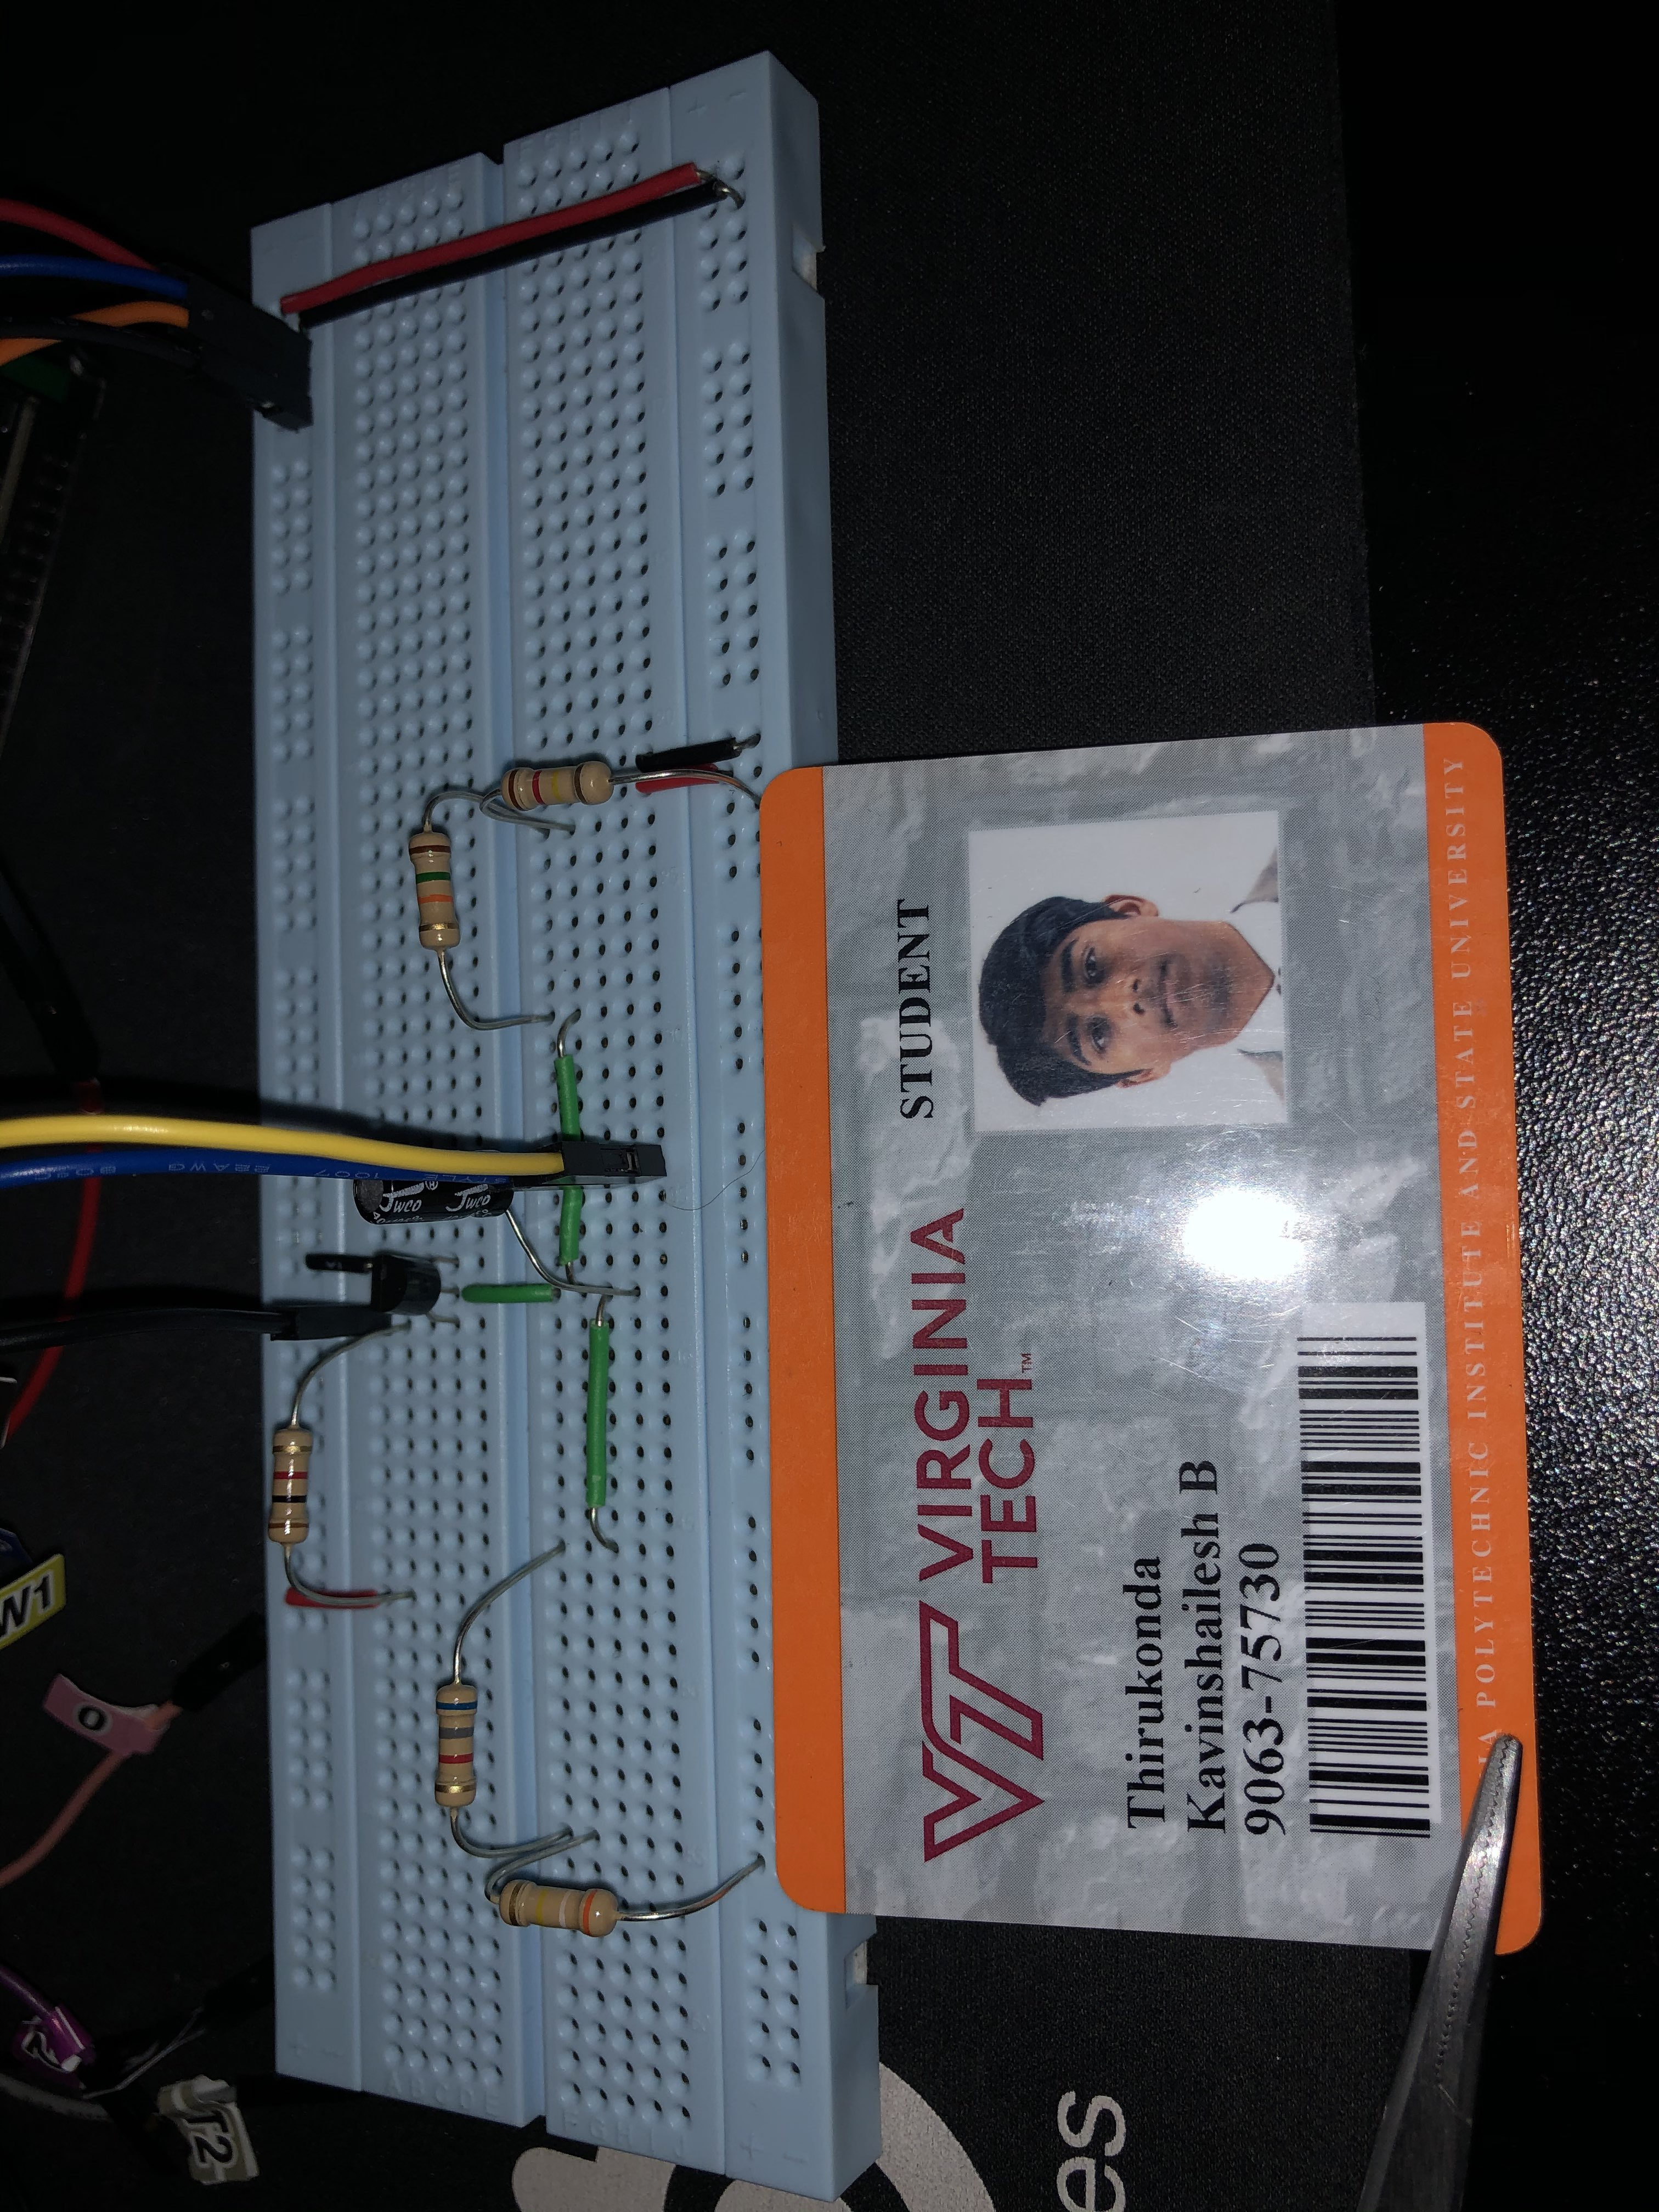
\includegraphics[height = .6\textwidth, width = .75\textwidth]{circuit.jpg}}
    \end{center}
\end{enumerate}
\end{enumerate}
\end{document}
